\chapter{METHODOLGIES \& IMPLEMENTATION}

This section of the thesis aims to provide a clear explanation of how the re-implementation was conducted in C. Providing all the steps taken in this attempt, with as much technical detail as possible and referencing appropriate sections of the original paper and code.

\section{Data structures, and Initial Parse Trees}
\subsubsection{Data Structures}
During this process of re-implementation, 2 structures were initialised. Structures are a way to group several related variables into one place in C \cite{w3schoolStructuresStructs2025}. One structure to represent a node in the parse trees, and another structure to hold and reference each parse tree.
\begin{figure}[H]

    \begin{tcolorbox}[title=Nodes Structure for storing trees, colback=white, colframe=black]
        \begin{lstlisting}[
            language=C,
            numbers=left,
            stepnumber=1,
            numbersep=5pt,
            xleftmargin=1.5em,
            frame=none
        ]
        typedef struct nodes{
            int capacity;
            int count;
            struct node **rootNodes;
        } Nodes;
        \end{lstlisting}

    \end{tcolorbox}

\caption{Data Structure to store and track trees}
\label{fig:Data_Structures1}
\end{figure}

Figure \ref{fig:Data_Structures1} shows the structure $Nodes$, used to hold all the parse trees. It has variables called \texttt{rootNodes}, which is a list containing pointers to the roots of all the parse trees. Now, as this implementation is in C and memory management is a dynamic and manual process, this structure holds 2 more variables \texttt{capacity} and \texttt{count}. Both of these variables are integers that are used to help manage the size of \texttt{rootNodes}. Variable \texttt{capacity} tracks the number of root node pointers \texttt{rootNodes} can currently hold, and variable $count$ tracks the number of actual root node pointers $rootNode$ currently has.

\begin{figure}[H]

    \begin{tcolorbox}[title=Node Structure to build each tree, colback=white, colframe=black]

        \begin{lstlisting}[
            language=C,
            numbers=left,
            stepnumber=1,
            numbersep=5pt,
            xleftmargin=1.5em,
            frame=none
        ]
        typedef struct node{
            int capacity;
            char character;
            struct node *parent;
            int t_label;
            int num_child;
            int pos;
            struct node **children;
        } Node;
        \end{lstlisting}
    \end{tcolorbox}

\caption{Data Structure to build each tree}
\label{fig:Data_Structures2}
\end{figure}


Figure \ref{fig:Data_Structures2} shows the structure $Node$, used for each individual node in the trees. It has 7 variables inside it. 
\begin{itemize}
    \item \texttt{character}: stores a C character if the node is a leaf/terminal node, else a null character if the node is a non-terminal.
    \item  \texttt{t\_label}: stores an integer. The integer is a positive value if the node is a non-terminal, else -1 if it is a terminal.
    \item \texttt{parent}: hold a pointer to the current node's parent, which is a $Node$ as well. If root, parent is a null pointer.
    \item \texttt{pos}: is an integer which represents the index of the current node when the parse trees are initially constructed for all terminal nodes. For non-terminal nodes, it will be a null value.
    \item \texttt{children}: hold a list of pointer, which point to $Node$.
    \item \texttt{capacity}: current size of the list $children$. 
    \item \texttt{num\_child}: current number of $Node$(s) pointer in list \texttt{children}.
\end{itemize}

\subsubsection{t\_id}
\begin{figure}[H]
    \begin{lstlisting}[
        language=C,
        numbers=left,
        stepnumber=1,
        numbersep=5pt,
        xleftmargin=1.5em,
        frame=none
    ]
    // Making tid global
    extern int *tid;
    tid = calloc(1, sizeof(int));
   \end{lstlisting}
\caption{Initialising a global tid variable}
\label{fig:globalTid}
\end{figure}

An global varible, \texttt{tid} was use to keep track of node non-terminal node labelling. It is incremented each time a new non-terminal is created and a tid is assigned. The \texttt{tid} is stored in \texttt{t\_label} of the node. Noting it is not used to assign \text{t\_label} of root nodes, as all root nodes have label 0. 

\section{Building Initial parse trees}
This part of the thesis is derived from section III-A of the original paper \cite{kulkarniLearningHighlyRecursive2021}. Using the 2 structures described, next, the initial parse trees were built. First, we build the $Nodes$ structure, which houses all the parse tree pointers. 
This is done by using C's built-in dynamic memory function $malloc$, where $capacity$ was set randomly to 4, $count$ to 0, as it does not house any parse tree pointers yet, and list $rootNodes$ was given enough memory to house 4 $Node$ pointers, where 4 is the current $capacity$. 

\begin{figure}[H]
    \begin{lstlisting}[
        language=C,
        numbers=left,
        stepnumber=1,
        numbersep=5pt,
        xleftmargin=1.5em,
        frame=none
    ]
    // Keeping track of all root trees (each string in example file)
    Nodes *root_trees= malloc(sizeof(Nodes)); 
    root_trees->capacity = 4; // randomly assigned
    root_trees->count = 0;
    root_trees->rootNodes= malloc(root_trees->capacity * sizeof(Node*));

    \end{lstlisting}

\caption{building of Nodes Structure}
\label{fig:rootNodes}
\end{figure}

Next, the file containing all the valid example strings is read as standard. Refer to figure \ref{fig:buildeachParseTree}, then from the top of the file, each valid string is read and each naive flat parse tree is built one by one. This is done by, looping through all the valid string and building a root node $t_0$. Then for each strings, looping through each character, builing a node to house this character. The doing appropriate assignings to make this character node a child of the root node. After each tree is built, the pointer to the tree's root if given and housed in \texttt{root\_trees} from figure \ref{fig:rootNodes}. 


\subsection{Memory management}

As the number of valid example strings and the length of each example string are not pre-determined, the number of \texttt{Nodes} (each parse tree), and the number of leaf nodes each non-terminal root node is going to is also non-determined. This means memory has to be allocated dynamically. To do this, two functions are used: one function to check and increase memory allocated to \texttt{root\_nodes} in \texttt{Nodes}, and another to check and increase memory allocated to \texttt{children} in \texttt{Node}. Both these functions check the \texttt{capacity} of their respective structures, and if \texttt{count} for \texttt{Nodes} and \texttt{num\_child} for \texttt{Node} equals \texttt{capacity}, they increase the memory allocated to their respective lists by 1.5 times the \texttt{capacity}, updating other variables appropriately. Function code in the appendix \ref{fig:capacityChangeCode}

\vspace{\baselineskip}
Since memory is being assigned dynamically, it also has to be freed dynamically. To help with this, a function is used. This helper function is given a node that does a depth-first search (DFS), and frees nodes as it searches, working its way bottom up. This is used to free memory as needed throughout, and all memory at the end. Refer to appendix \ref{fig:freeNodes}


\begin{figure}[H]
    \begin{lstlisting}[
        language=C,
        numbers=left,
        stepnumber=1,
        numbersep=5pt,
        xleftmargin=1.5em,
        frame=none
    ]
    // Buffer to store the current example read.
    char *current_line = NULL; // 
    size_t line_buffer_len = 0;
    ssize_t read_line_len = 0;
    
    //Read line by line until the end of the file has been reached.
    while((read_line_len = getline(&current_line, &line_buffer_len, file_ptr)) != -1){

        current_line[read_line_len - 1] = '\0';

        //building the naive parse tree for each string
        // So the root node for each parse tree
        Node *current_tree = build_basic_node(); // appendix 6.1
        current_tree->capacity = 10; // randomly assigned
        current_tree->t_label = 0;
        current_tree->children = calloc(current_tree->capacity, sizeof(Node*));

        // Going through all the characters in the string 1 by 1. 
        // Building the terminal nodes, assign a character value to the node.
        for(int i = 0; i < (read_line_len - 1); i ++ ){
            Node * node = build_basic_node();
            node->parent = current_tree;
            node->character = current_line[i];
            node->pos = i;
            current_tree->children[current_tree->num_child] = node;
            current_tree->num_child ++;
            // checking current trees' capacity
            // increase appropriately if needed
            check_node_capacity(current_tree);

        }

        // Check current capacity of the root node.
        // Increase appropriately
        root_trees->rootNodes[root_trees->count] = current_tree;
        root_trees->count = root_trees->count + 1;
        check_nodes_capacity(root_trees);

    }
    
    // Free buffer
    free(current_line);

\end{lstlisting}

\caption{Building each initial parse tree}
\label{fig:buildeachParseTree}
\end{figure}

\subsection{Pre-tokenisation}


\begin{figure}[H]
    \begin{lstlisting}[
        language=C,
        numbers=left,
        stepnumber=1,
        numbersep=5pt,
        xleftmargin=1.5em,
        frame=none
    ]
     // Step 2: Toggling pre-tokenisation
     // Section III-E of the Original paper
     int tokenise = 0;

     if(tokenise){
        for (int i = 0; i < root_trees->count; i ++){
            pre_tokenise(root_trees->rootNodes[i]);
        }
     }



    \end{lstlisting}

\caption{Pre-tokenisation of each root node}
\label{fig:pre-tokenise in main loop}
\end{figure}
    
After the initial parse trees were built, pre-tokenisation, as described in Section~III-A of the original paper \cite{kulkarniLearningHighlyRecursive2021}, was implemented. This process involved looping through each parse tree in the \texttt{Nodes} structure and, for each parse tree, iterating through all its leaf nodes. The goal was to group consecutive sequences of leaf nodes belonging to the same class and place them under an intermediate node positioned between the root node and the sequence of leaf nodes—also referred to as a label node. The pre-tokenisation of each parse tree was encapsulated within a dedicated function, which performed pre-tokenisation given the root node $t_0$ of a parse tree. 

\vspace{\baselineskip}
Given a root node $t_0$, the function first detaches all of its children ($c_0, c_1, \dots, c_n$) from the root. This is achieved by assigning an empty list to the root’s children list pointer and storing the original list of children ($c_0, c_1, \dots, c_n$) in a temporary variable. It then creates a new intermediate non-terminal label node $t_i$ and began iterating through the detached children. The function takes the first child node $c_0$, assigns it as a child of $t_i$, and keep track of its class and the number of nodes assigned to $t_i$ (i.e., the length of the current sequence of the same class). It then continues through $c_1, c_2, \dots, c_n$, and as long as the current child $c_i$ belonged to the same class, it continued assigning it as a child of $t_i$.  

\vspace{\baselineskip}
When a punctuation mark or a node $c_i$ of a different class was encountered, and $t_i$ contains a sequence of more than one child, the function assigns increments and assign $t_i$ a \texttt{tid}. Then assign $t_i$ as a child of the root $t_0$ and creates a new non-terminal node $t_j$ to begin a new sequence. This process is then repeated. If $t_i$ contains a sequence of length one when a class change occurrs, and a new sequence is about to begin, $t_i$ is dissolved, and the single child $c_p$ is directly linked to the root $t_0$. The process is then restarted with a new non-terminal label node $t_k$. The same approach is applied when punctuation marks are encountered.  

\vspace{\baselineskip}
Essentially, this process ensures that intermediate non-terminal label nodes are only created for leaf nodes of the same class that form consecutive sequences of length two or greater. Refer to Appendix~\ref{fig:Pre_tokeniser} and Appendix~\ref{fig:pre_tokenise helper} for the implementation details.


\begin{figure}[H]
\centering
\begin{tikzpicture}[
    node distance=10mm,
    every node/.style={align=center}
]

% Left tree
\node (lefttree) {
\begin{tikzpicture}[
    level distance=10mm,
    sibling distance=4mm,
    every node/.style={draw=none, inner sep=1pt, font=\small, anchor=base},
    edge from parent/.style={draw}
]
\node {$t_0$}
    child {node {w}}
    child {node {h}}
    child {node {i}}
    child {node {l}}
    child {node {e}}
    child {node {\textvisiblespace}}
    child {node {L}}
    child {node {\textvisiblespace}}
    child {node {=}}
    child {node {=}}
    child {node {\textvisiblespace}}
    child {node {n}};
\end{tikzpicture}
};


% Right tree
\node[right=of lefttree] (righttree) {
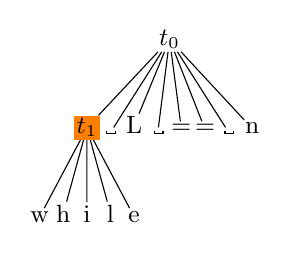
\begin{tikzpicture}[
    level distance=12mm,
    sibling distance=3mm,
    every node/.style={draw=none, inner sep=1pt, font=\small, anchor=base},
    edge from parent/.style={draw}
]
\node {$t_0$}
    child {node[fill=orange] {$t_1$}
        child {node {w}}
        child {node {h}}
        child {node {i}}
        child {node {l}}
        child {node {e}}
    }
    child {node {\textvisiblespace}}
    child {node {L}}
    child {node {\textvisiblespace}}
    child {node {=}}
    child {node {=}}
    child {node {\textvisiblespace}}
    child {node {n}};
\end{tikzpicture}
};
\end{tikzpicture}

\caption{Visualisation of adding a intermediate node, and tokenisation}
\label{fig:addingInterVis}
\end{figure}



\subsection{MERGEALLVALID}

Following the explanation provided in Section~III-A of the original paper \cite{kulkarniLearningHighlyRecursive2021}, the function MERGEALLVALID was implemented. After pre-tokenisation, another loop is executed that iterates through each parse tree $T_i$ and calls the MERGEALLVALID function on it.


\begin{figure}[H]
    \begin{lstlisting}[
        language=C,
        numbers=left,
        stepnumber=1,
        numbersep=5pt,
        xleftmargin=1.5em,
        frame=none
    ]
     // Step 3: MergeAllValid 
     // Section III-A of Original paper
     for( int i = 0; i < root_trees -> count; i++){
        merge_all_valid(root_trees->rootNodes[i], root_trees);
     } 
    \end{lstlisting}

\caption{MergeAllValid call}
\label{fig:pre-tokenise in main loop}
\end{figure}

Referencing Appendix~\ref{fig:MergeAllValid function code}, once the function was given a parse tree $T_i$ with root $t_0$, it iterates through all its children, which are either leaf nodes ($c_i$) or non-terminal label nodes ($t_i$). For each child node $c_i / t_i$, the function then loops from the current node $c_{i+1} / t_{i+1}$ to the final node $c_n / t_n$, effectively generating all combinations of two child nodes ($t_a / c_a$ and $t_b / c_b$). This looping process is executed twice.

\vspace{\baselineskip}
While ignoring whitespace nodes as potential $t_a / c_a$ or $t_b / c_b$, the first time looping, it checks for pair of nodes $t_a / c_a$ and $t_b / c_b$ that produce the same string when concatenated. String concatenation, given a node, is a done by doing a depth-first search (DFS) traversal to the leaf nodes, retrieving each character, and storing it in a buffer (see Appendix~\ref{fig:Stirng Concatenate}).

\vspace{\baselineskip}
If $t_a / c_a$ and $t_b / c_b$ produces identical concatenated strings, the function merged both pairs ($t_a / c_a$ and $t_b / c_b$). This merging process is carried out through another function (Appendix~\ref{fig:Merging Same nodes}), which creates two new intermediate nodes with identical labels (same \texttt{t\_label}) if the two child nodes being compared are leaf nodes ($c_a$ and $c_b$). Otherwise, if the two nodes were non-terminals ($t_a$ and $t_b$), the function simply updated their \texttt{t\_label} values accordingly, assigning the smaller label value to the larger non-terminal.

\vspace{\baselineskip}
Once all identical string-producing nodes had been processed, ARVADA iterated through all the parse trees again, generating combinations of two child nodes once more—this time dealing with every $t_a / c_a$ and $t_b / c_b$ pair that produced different concatenated strings. Before merging these nodes, several checks were performed. The function first checkes for whitespace nodes, but this time to exclude nodes that produced identical strings. It also checked whether the nodes under consideration, $t_a$ and $t_b$, had already been merged. This was determined by verifying if $t_a$ and $t_b$ shared the same non-negative \texttt{t\_label}.

\vspace{\baselineskip}
After this, to process all not identical nodes, a different check is done to merge.If $t_a / c_a$ could replace $t_b / c_b$ in all parse trees and still produce valid concatenated strings—and vice versa ($t_b / c_b$ replacing $t_a / c_a$)—then the merge was executed. The procedure for performing this merge was described in the string replacement section of the original paper. The merging of two different node sequences was conducted in a similar manner to the merging of identical sequence nodes, as explained in the merging section.


In this re-implementation, because the \texttt{MERGEALLVALID} function first handles identical subtrees, two different merge functions were implemented: a general merge function (Appendix~\ref{fig:Gerenal merge function}) and a more specialised merge function used exclusively within \texttt{MERGEALLVALID} (Appendix~\ref{fig:Merging Same nodes}).

\vspace{\baselineskip}
The general merge function is used in \texttt{MERGEALLVALID} and can also be applied after the bubbling process in \texttt{CHECKBUBBLES}. This function takes two nodes as input, and if either of the given nodes is a terminal (leaf) node, it immediately introduces a non-terminal intermediate node—effectively adding an additional layer to the tree structure (similar to the operation performed during pre-tokenisation). This intermediate node is then used for re-labelling. Refer to Figure~\ref{fig:addingInterVis} for a visualisation of adding an intermediate node.

\begin{figure}[H]
\centering
\begin{tikzpicture}[
    node distance=10mm,
    every node/.style={align=center}
]

% Left tree
\node (lefttree) {
\begin{tikzpicture}[
    level distance=12mm,
    level 1/.style={sibling distance=5mm},
    level 2/.style={sibling distance=2mm},
    sibling distance=4mm,
    every node/.style={draw=none, inner sep=1pt, font=\small, anchor=base},
    edge from parent/.style={draw}
]
\node {$t_0$}
    child {node {$t_1$}
        child {node {w}}
        child {node {h}}
        child {node {i}}
        child {node {l}}
        child {node {e}}
    }
    child {node {\textvisiblespace}}
    child {node[fill=yellow] {$t_2$}
        child {node {t}}
        child {node {r}}
        child {node {u}}
        child {node {e}}
    }
    child {node {\textvisiblespace}}
    child {node {\&}}
    child {node {\&}}
    child {node {\textvisiblespace}}
    child {node[fill=yellow] {$t_3$}
        child {node {f}}
        child {node {a}}
        child {node {l}}
        child {node {s}}
        child {node {e}}
    };
\end{tikzpicture}
};

% Right tree
\node[right=of lefttree] (righttree) {
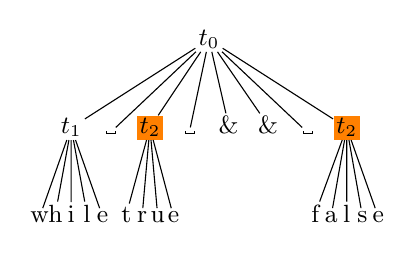
\begin{tikzpicture}[
    level distance=12mm,
    level 1/.style={sibling distance=5mm},
    level 2/.style={sibling distance=2mm},
    sibling distance=3mm,
    every node/.style={draw=none, inner sep=1pt, font=\small, anchor=base},
    edge from parent/.style={draw}
]
\node {$t_0$}
    child {node {$t_1$}
        child {node {w}}
        child {node {h}}
        child {node {i}}
        child {node {l}}
        child {node {e}}
    }
    child {node {\textvisiblespace}}
    child {node[fill=orange] {$t_2$}
        child {node {t}}
        child {node {r}}
        child {node {u}}
        child {node {e}}
    }
    child {node {\textvisiblespace}}
    child {node {\&}}
    child {node {\&}}
    child {node {\textvisiblespace}}
    child {node[fill=orange] {$t_2$}
        child {node {f}}
        child {node {a}}
        child {node {l}}
        child {node {s}}
        child {node {e}}
    };
\end{tikzpicture}
};
\end{tikzpicture}
\caption{Visualisation of re-labelling}
\label{fig:relabelingVis}
\end{figure}

\vspace{\baselineskip}
The more specialised merge function, used only in \texttt{MERGEALLVALID}, was designed to handle cases where there are more than two identical leaf nodes directly linked to the root of a parse tree during the initial traversal. Consider the following example:

\begin{center}
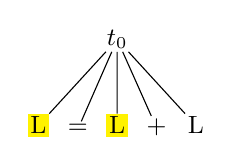
\begin{tikzpicture}[
    level distance=12mm,
    level 1/.style={sibling distance=5mm},
    level 2/.style={sibling distance=2mm},
    sibling distance=3mm,
    every node/.style={draw=none, inner sep=1pt, font=\small, anchor=base},
    edge from parent/.style={draw}
]
\node {$t_0$}
    child {node[fill=yellow] {L}}
    child {node {=}}
    child {node[fill=yellow] {L}}
    child {node {+}}
    child {node {L}};
\end{tikzpicture}

$\big\downarrow$

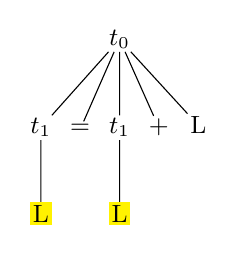
\begin{tikzpicture}[
    level distance=12mm,
    level 1/.style={sibling distance=5mm},
    level 2/.style={sibling distance=2mm},
    sibling distance=3mm,
    every node/.style={draw=none, inner sep=1pt, font=\small, anchor=base},
    edge from parent/.style={draw}
]
\node {$t_0$}
    child {node {$t_1$}
        child {node[fill=yellow] {L}}
    }
    child {node {=}}
    child {node {$t_1$}
        child {node[fill=yellow] {L}}
    }
    child {node {+}}
    child {node {L}};
\end{tikzpicture}
\end{center}

The highlighted nodes represent the nodes under consideration in the loop. The first time two identical direct leaf nodes are found, the process is straightforward: both nodes are wrapped under newly created intermediate nodes with the same label, updating the tree structure accordingly. However, since the loop continues without restarting after the modification, a situation may arise as shown below:

\begin{center}
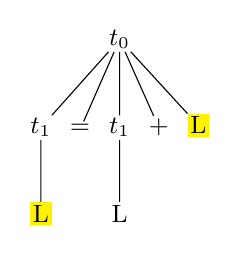
\begin{tikzpicture}[
    level distance=12mm,
    level 1/.style={sibling distance=5mm},
    level 2/.style={sibling distance=2mm},
    sibling distance=3mm,
    every node/.style={draw=none, inner sep=1pt, font=\small, anchor=base},
    edge from parent/.style={draw}
]
\node {$t_0$}
    child {node {$t_1$}
        child {node[fill=yellow] {L}}
    }
    child {node {=}}
    child {node {$t_1$}
        child {node {L}}
    }
    child {node {+}}
    child {node[fill=yellow] {L}};
\end{tikzpicture}
\end{center}

Here, the two identical nodes remain leaf nodes, but only one of them is still directly connected to the root. Therefore, to merge these nodes correctly, only the one directly attached to the root requires an intermediate node. The specialised merge function handles this case by performing an additional check to determine whether the nodes are directly connected to the root before merging.

\section{String replacement}

For merging 2 different nodes,

\section{Oracle and other testing}

\subsection{Bubbling}

This section of ARVADA has not been implemented yet. Hence, further future work is required to complete the re-implementation.


